\documentclass[./\jobname.tex]{subfiles}
\begin{document}

\section{Experimental Design}
This section gives an overview on how the subsequent experiments are conducted. An integral part of solver comparison is to define a testbed that holds example problems with a known analytical solution. Further, a quality measurement must be defined that compares the numerical to the analytical solution. Since the memory consumption and the solving time is of interest, a robust method to measure these characteristics is needed. The baseline for all experiments is the \gls{fem} solver NGSolve \cite{schoberl_ngsolvengsolve_2020}. 

\subsection{Testbed}
\label{chap:testbed_description}
The testbed is a collection of multiple two-dimensional scalar \gls{pde}s that are analytically solved such that $u_{ext}(\mathbf{x}): \mathbb{R}^2 \rightarrow \mathbb{R}$ is a solution to the underlying PDE. The equations used here are a mixture of different testbeds. Specifically, the equations \gls{pde} 2 and \gls{pde} 3 are picked from the testbed in \cite{chaquet_using_2019},  \cite{tsoulos_solving_2006} and \cite{panagant_solving_2014}. The more complex equations are taken from the National Institute of Standards and Technology (NIST) website \cite{mitchell_nist_2018} that provides benchmarking problems for \gls{fem} solvers with adaptive mesh refinement methods. The other equations 0A, 0B and 8 are specially created to show different properties of the solver. 

\begin{table}[h]
	\centering
	\noindent\adjustbox{max width=\linewidth}{
		\begin{tabular}{|c|c|}
			
			\hline
			\rowcolor[HTML]{\farbeTabA}
			
			PDE Abbreviation & Description \\ \hline
			
			\multilinecell{PDE 0A: Gauss Kernel} & \multilinecell{superposition \\ of 5 \gls{gak}} \\ \hline
			\multilinecell{PDE 0B: Gauss\\ Sine Kernel} & \multilinecell{superposition \\ of 3 \gls{gsk}} \\ \hline
			\multilinecell{PDE 1: Polynomial 2D} & \multilinecell{polynomial of \\order 20} \\ \hline
			\multilinecell{PDE 2: Chaquet PDE 1} & \multilinecell{slightly curved \\ e-function} \\ \hline
			\multilinecell{PDE 3: Chaquet PDE 3} & \multilinecell{polynomial of \\ order 2} \\ \hline
			\multilinecell{PDE 4: Sine Bump 2D} & \multilinecell{homogeneous sine  \\on unit square} \\ \hline
			\multilinecell{PDE 5: Arctan \\Circular Wave Front} &\multilinecell{ arctan with \\steep gradient} \\ \hline
			\multilinecell{PDE 6: Peak 2D} & \multilinecell{sharp Gauss function \\ with steep gradient} \\ \hline
			\multilinecell{PDE 7: Boundary \\Line Singularity} & \multilinecell{root function defined \\ on $x \in \mathbb{R}^+$} \\ \hline
			\multilinecell{PDE 8: Interior \\ Point Singularity} & \multilinecell{root function with \\ singularity at $[0.5, 0.5]$} \\ \hline
			\multilinecell{PDE 9: Arctan Wave Front \\Homogeneous Boundary\\ Conditions 2D} & \multilinecell{arctan oscillation\\  on diagonal of \\ unit square} \\ \hline
		\end{tabular}
	}
	\unterschrift{Table of the testbed \gls{pde}s used in this paper.}{}{}
	\label{tab:testbed_pdes}
\end{table}

\subsection{Software Architecture}
\label{chap:software_architecutre}
To simplify the preparation, execution and evaluation of the experiments, a comprehensive software architecture is defined. A simplified class diagram, without any methods and attributes is shown in figure \ref{fig:uml_class_small} below. The architecture is organised in four main segments: Optimisation Algorithm (OptAlgo), Kernels, Testbed and Post Processing (post\textunderscore proc)

\begin{figure}[h]
	\centering
	\noindent\adjustbox{max width=\linewidth}{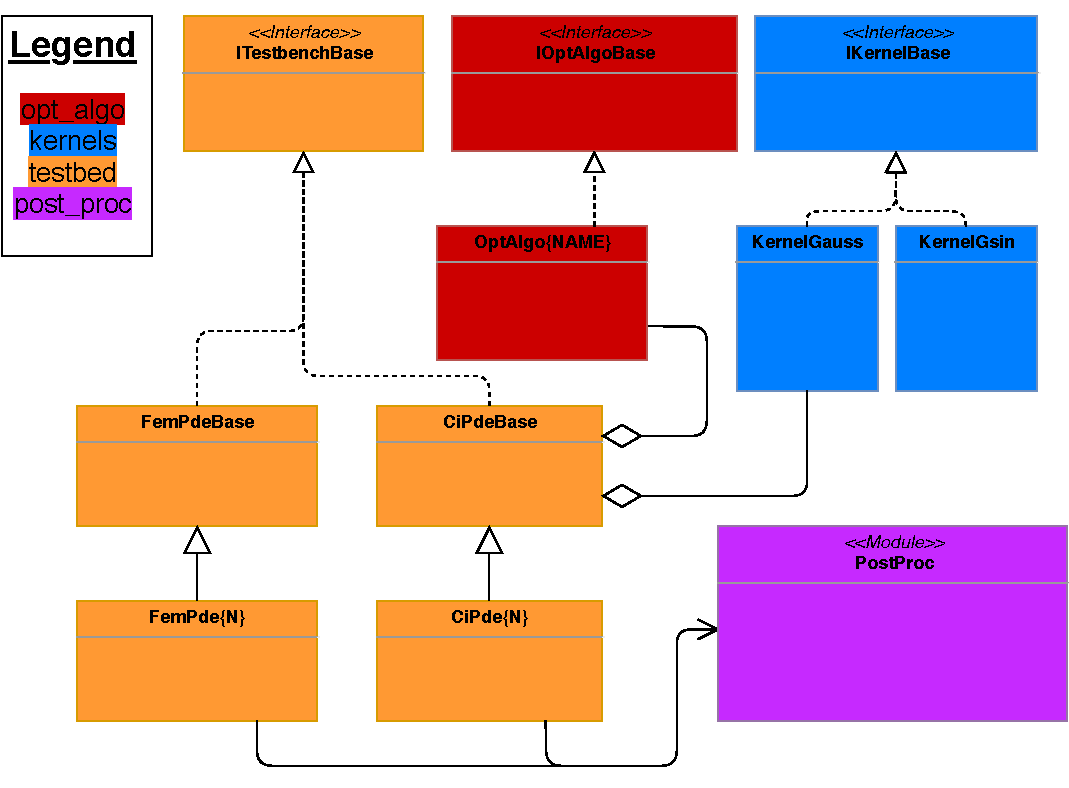
\includegraphics[width=1\textwidth]{../../code/uml_diag/testbench_uml_class_small.pdf}
	}
	\unterschrift{This reduced \gls{uml} class diagram gives an overview of the testbed design and its interfaces and classes.}{}{}
	\label{fig:uml_class_small}
\end{figure}

\subsection{Performance Metric} 
\label{chap:metric}
In order to scientifically compare the results produced by the different solvers, some metrics are necessary. Three important solver-properties are measured: the execution time, the memory usage and the quality of the numerical solution. Although the fitness function is the criterion that is optimised, it is not applicable as an objective quality measure. As \cite{chaquet_using_2019} describe, it depends on multiple factors:
\begin{itemize}
	\item user-defined parameters $\xi$ and $\phi$ 
	\item the formulation of the \gls{pde} 
	\item number of collocation points used 
	\item number of kernels used
\end{itemize}
Thus, \cite{chaquet_using_2019} define a new quality measurement based on the \gls{rmse} over the collocation points as seen in equation \eqref{eq:rmse_chaquet}. 
\begin{equation}
\label{eq:rmse_chaquet}
\begin{split}
RMSE^2 = \frac{1}{(n_C + n_B)} \\ \left[\sum_{i=1, \mathbf{x}_i \in C}^{n_C} \right. \left|\left| u(\mathbf{x}_i) - u_{ext}(\mathbf{x}_i) \right|\right|^2 \\ + \left. \sum_{j=1, \mathbf{x}_j \in B}^{n_B} \left|\left| u(\mathbf{x}_j) - u_{ext}(\mathbf{x}_j) \right|\right|^2 \right]
\end{split}
\end{equation}
This quality criterion has three inherent issues. At first, it firmly depends on the number of collocation points used. Further, only the quality on the collocation points is measured and not in between. However, a good solution fits not only these discrete points, but the whole domain. This is called an aliasing error. An approximation can fit the points, without correctly representing the space between them. This is shown in the following figure \ref{fig:aliasing error}.

\begin{figure}[h]
	\centering
	\noindent\adjustbox{max width=0.8\linewidth}{
		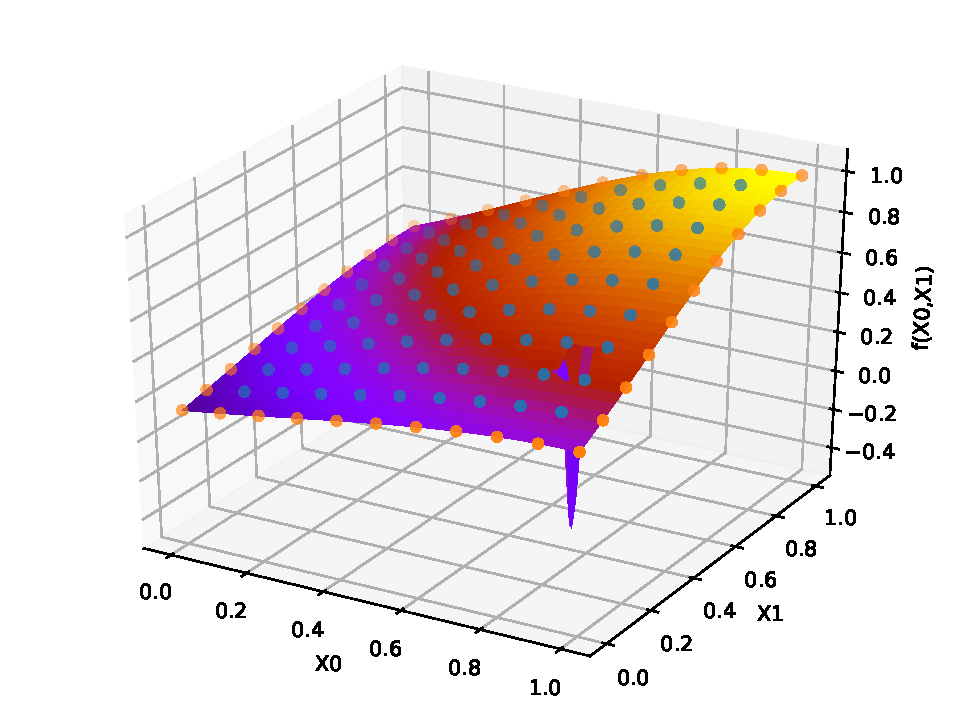
\includegraphics[width=\textwidth]{../img/pdf/aliasing_error.pdf}
	}
	\unterschrift{Aliasing Error: sharp inaccuracies in between collocation points}{}{}
	\label{fig:aliasing error}
\end{figure}
Finally, the \gls{fem} method doesn't use collocation points, so this quality measurement could not be calculated. This leads to the quality measurement formulation used in this thesis: the L2 norm defined for functions as denoted in equation \eqref{eq:quality_measurement}. This measures the distance between the analytical solution and the numerical approximation.  
\begin{equation}
\label{eq:quality_measurement}
\left|\left|u_{ext} - u_{apx}\right|\right| = \sqrt{\int_{\Omega} (u_{ext}(\mathbf{x}) - u_{apx}(\mathbf{x}))^2 dx}
\end{equation}
\newpage
Although this integral is numerically evaluated, the discretisation is much finer than the resolution of the collocation points used in the fitness function - thus also taking the areas between these points into account.\\
To validate the results, a statistical significance test is performed. The test function is based on the Wilcoxon test at a significance level of $\alpha = 0.05$. To decide if the results are better or worse, the mean and the median are compared. If both are smaller, the results are better. Contrary, if both are larger, the results are worse. If only one of the values is smaller, the results are undecided. 

\subsection{Baseline: NGSolve}
\label{chap:fem_baseline_results}
NGSolve \cite{schoberl_ngsolvengsolve_2020} is a state of the art \gls{fem} solver that is in part developed and maintained by numerous well-known institutes such as the Vienna University of Technology, the University of Göttingen and the Portland State University. 
\subsubsection{Setup}
At first the \gls{pde}s must be transformed into their corresponding weak form. As all testbed problems are Poisson equations and only differ in their algebraic sign and inhomogeneous part, the weak form is similar for all problems. Referring to equation \eqref{eq: weak form}, the terms $\vec{b} = 0$ and $c = 0$, thus these parts vanish. The matrix $A$ is either $\begin{bsmallmatrix} 1 & 0 \\ 0 & 1 \end{bsmallmatrix}$ or with a negative sign $\begin{bsmallmatrix} -1 & 0 \\ 0 & -1 \end{bsmallmatrix}$ as only the non-mixed second order derivatives occur in the equations. This results in the weak form as presented in equation \eqref{eq: weak form testbed}, where f is the inhomogeneous part of the \gls{pde}.
\begin{equation}
\label{eq: weak form testbed}
\int_{\Omega} \nabla u^T \nabla v dV = \int_{\Omega} f v dV
\end{equation}
To enhance the performance of NGSolve, static condensation is turned on. Further, a multigrid preconditioner is used. All problems are approximated by second order polynomials. The automatic mesh refinement is performed until a maximum of $5 \cdot 10^4$ \gls{dof} is reached. To properly interpret the results, 20 replications for each problem are performed. This is only needed for time and memory usage, the solution itself is not a random variable. To further reduce memory usage, the GUI of NGSolve is switched off. 
\subsubsection{Result}
With the parameters described above, the following results are produced. The solving time as well as the memory usage are displayed in the boxplots \ref{fig:_fem_time_boxplot} and \ref{fig:_fem_mem_boxplot}, respectively. In general, the solving time ranges from 2.5 to 5.0 seconds at about 50 to 80 Mbyte of memory. Only problem 3 stands out as a notable exception. To keep the diagram within a readable scale, this \gls{pde} is omitted and plotted in a separate figure. Table \ref{tab:fem_sol_quality} presents the achieved distances between the exact and the approximated solutions. On \gls{pde} 3 the best numerical quality is achieved. The problem \gls{pde} 7 only needs around 2.5 seconds to be solved. A reason could be that the solution only depends on one variable and the derivative with respect to y evaluate to zero $\frac{\partial u}{\partial y} = 0$ and thus vanishes. This does not effect the memory usage, since all $5 \cdot 10^4$ \gls{dof} must be created to terminate. 

\begin{table}[h]
	\centering
	\noindent\adjustbox{max width=\linewidth}{
		\begin{tabular}{|c|c|}
			
			\hline
			\rowcolor[HTML]{\farbeTabA}
			
			Problem PDE & L2 Norm \\ \hline
			
			0A & $2.967 \cdot 10^{-5}$ \\ \hline
			0B & $1.071 \cdot 10^{-5}$ \\ \hline
			1  & $8.004 \cdot 10^{-7}$ \\ \hline
			2  & $3.501 \cdot 10^{-8}$ \\ \hline
			3  & $1.680 \cdot 10^{-9}$ \\ \hline
			4  & $4.764 \cdot 10^{-7}$ \\ \hline
			5  & $6.057 \cdot 10^{-6}$ \\ \hline
			6  & $1.908 \cdot 10^{-7}$ \\ \hline
			7  & $5.203 \cdot 10^{-5}$ \\ \hline
			8  & $3.237 \cdot 10^{-7}$ \\ \hline
			9  & $2.366 \cdot 10^{-7}$ \\ \hline
			
		\end{tabular}
	}
	\unterschrift{These are the results obtained by the \gls{fem} solver in terms of distance to the analytical solution.}{}{}
	\label{tab:fem_sol_quality}
\end{table}
\begin{figure}[h]
	\centering
	\noindent\adjustbox{max width=0.75\linewidth}{
		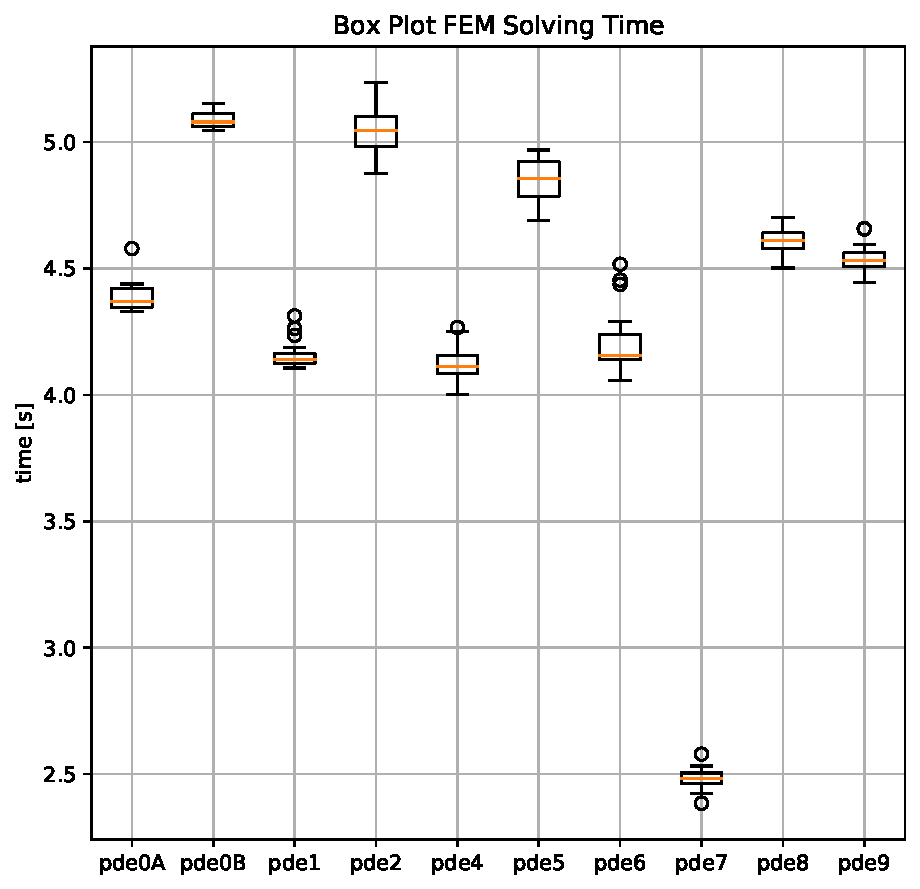
\includegraphics[width=\textwidth]{../../code/experiments/_experiment_fem_base/time_boxplot_pde_0a_0b_1_2_4_5_6_7_8_9.pdf}
	}
	\unterschrift{Boxplot: time (in seconds) needed to solve the testbed \gls{pde} (without \gls{pde}3)}{}{}
	\label{fig:_fem_time_boxplot}
\end{figure}

\begin{figure}[h]
	\centering
	\noindent\adjustbox{max width=0.75\linewidth}{
		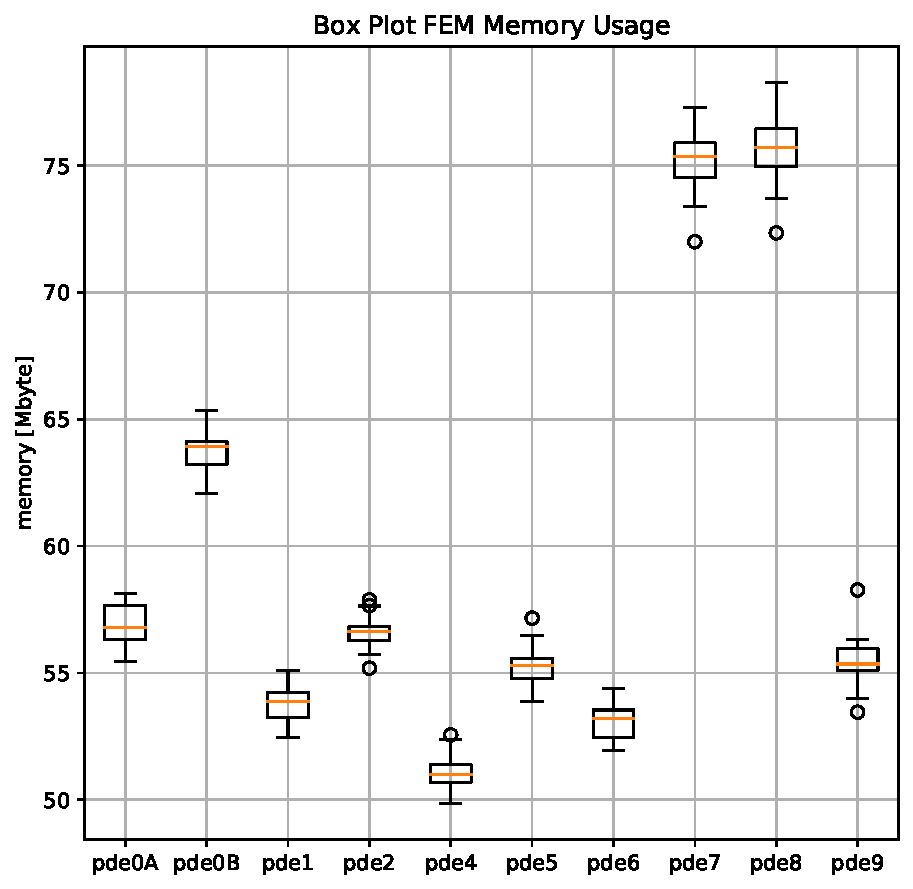
\includegraphics[width=\textwidth]{../../code/experiments/_experiment_fem_base/mem_boxplot_pde_0a_0b_1_2_4_5_6_7_8_9.pdf}
	}
	\unterschrift{Boxplot: memory (in Mbyte) needed to solve the testbed \gls{pde} (without \gls{pde}3)}{}{}
	\label{fig:_fem_mem_boxplot}
\end{figure}
The following figures \ref{fig:_fem_time_boxplot_pde3} and \ref{fig:_fem_mem_boxplot_pde3} show the boxplot of the time and memory consumption for the testbed \gls{pde} 3 with $5 \cdot 10^4$ \gls{dof}. Compared to the other equations, this problem takes longer to solve while also needing more memory: somewhere around 65.2 seconds at about 130 Mbyte. One possible explanation for that is the fundamental structure of solution. The exact solution to this problem is a polynomial of second order. This can be approximated perfectly by the \gls{fem} solver, since it also uses second order polynomials as basis functions. The mesh-refinement step takes more iterations to produce the $5 \cdot 10^4$ \gls{dof} as compared to the other testbed problems. In fact, since the numerical errors per finite element accumulate, more \gls{dof} should result in a larger approximation error. Figure \ref{fig:_dof_sweep_pde3} shows the performance metrics at different \gls{dof} budgets. The plot supports this hypothesis, that less \gls{dof} take less time and memory to solve the \gls{pde} and still end up with a better quality. 
\begin{figure}[h]
	\centering
	\noindent\adjustbox{max width=0.9\linewidth}{
		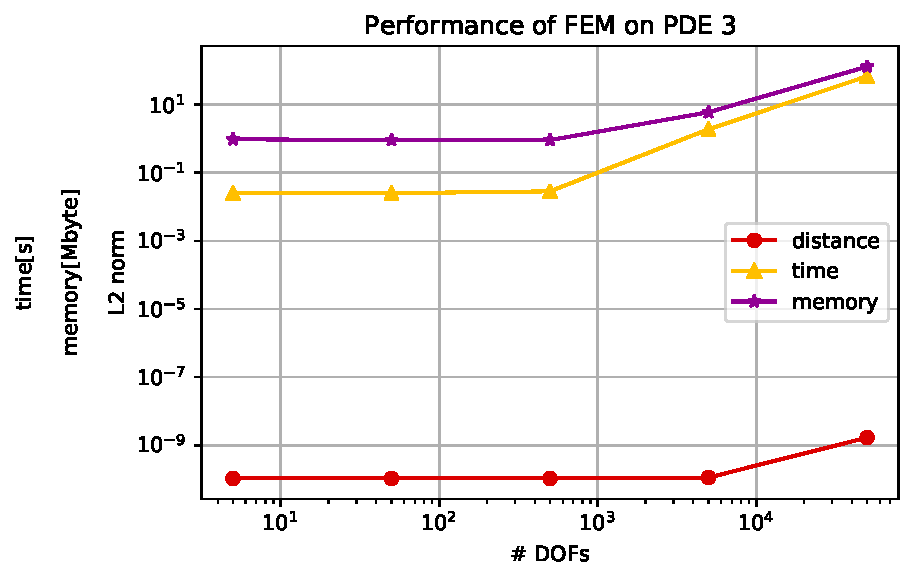
\includegraphics[width=\textwidth]{../../code/experiments/_experiment_fem_base/pde3_ndof.pdf}
	}
	\unterschrift{\gls{pde} 3 performance metrics at different \gls{dof} budgets.}{}{}
	\label{fig:_dof_sweep_pde3}
\end{figure}
\begin{figure}[h]
	\centering
	\begin{subfigure}[b]{0.5\linewidth}
		\centering
		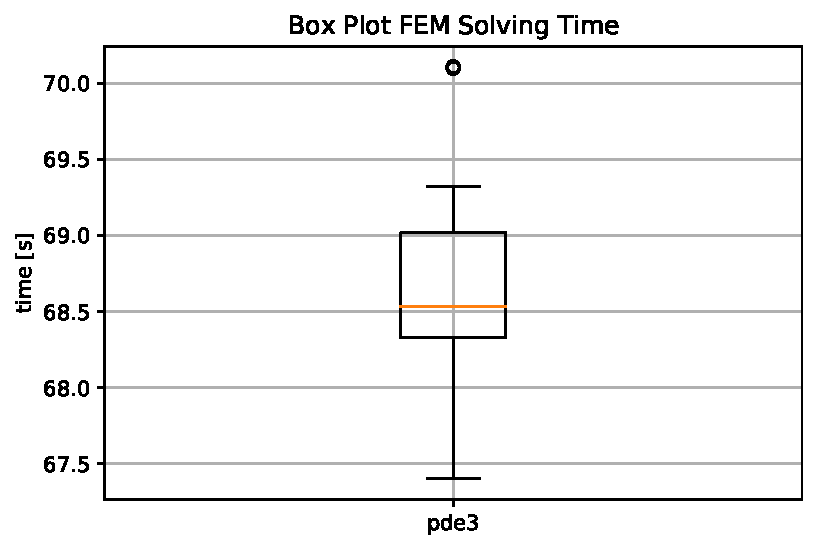
\includegraphics[width=1\textwidth]{../../code/experiments/_experiment_fem_base/time_boxplot_pde_3.pdf}
		\caption{Boxplot: time to solve testbed \gls{pde}3 at $5\cdot 10^4$ \gls{dof}.}
		\label{fig:_fem_time_boxplot_pde3}
	\end{subfigure}% 
	%
	\begin{subfigure}[b]{0.5\linewidth}
		\centering
		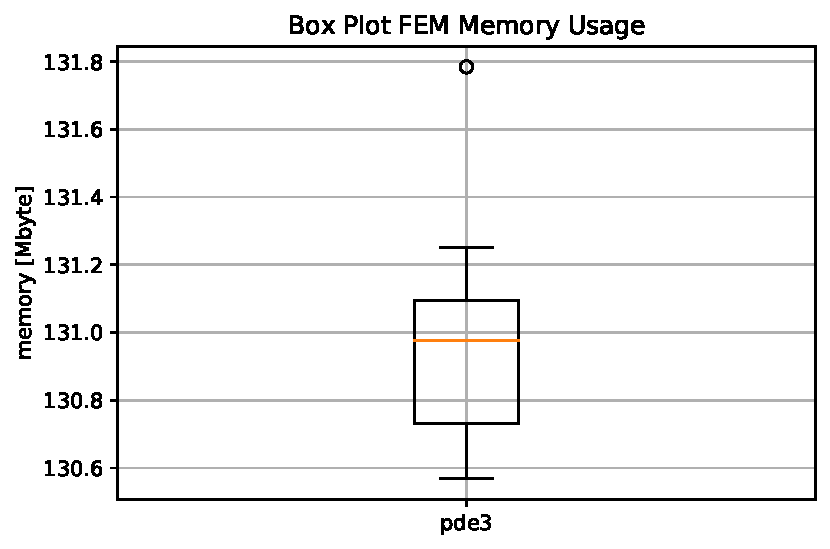
\includegraphics[width=1\textwidth]{../../code/experiments/_experiment_fem_base/mem_boxplot_pde_3.pdf}
		\caption{Boxplot: memory to solve testbed \gls{pde}3 at $5\cdot 10^4$ \gls{dof}.}
		\label{fig:_fem_mem_boxplot_pde3}
	\end{subfigure}%
	\unterschrift{Comparison of time and memory effort on \gls{pde} 3 at $5 \cdot 10^4$ \gls{dof}.}{}{}%
	\label{}
\end{figure}

\subsection{Default CI Parameter}
\label{chap:default_ci_param}
Typically, the performance of heuristic optimisation algorithms can be adjusted to specific testbed problems by tuning its parameters. For all further experiments the JADE algorithm is used. Similarly, the reported \gls{ci} solver has many parameters that could be adapted. However, adjusting every parameter in order to find the best combination is not an option, since that would take an extensive amount of computation time. Some parameters that might not have a great effect on the performance can be predefined. These values are determined by preliminary tests. If not stated otherwise, the following parameters from table \ref{tab:ci_parameter} are used in the subsequent experiments. 

The \gls{fem} solver terminates after it surpasses $5 \cdot 10^4$ \gls{dof}. The whole number of collocation points ($n_B + n_C$) is the equivalent for the \gls{ci} solver. Typically, fewer collocation points are used, since the evaluation time of the fitness function scales poorly with more points. \cite{chaquet_using_2019} use 100 equally spaced collocation points over the domain to solve the \gls{pde}. Here, 121 points are created. Figure \ref{fig:collocation_weight} shows the values of $\xi$ and $\varphi$. It further describes how the weighting factor emphasises the areas closer to the boundary. Typically, \gls{de} uses larger population sizes. \cite{mallipeddi_empirical_2008} describe an empirical study on choosing this parameter. They discuss the trade-off between premature convergence and computational effort. The results suggest that population sizes of $2\cdot dim$ are more likely to stagnate, but also converge faster. Since time is a critical resource for the \gls{ci}-solver, this population size is chosen. To account for the statistical influence, every setup is reevaluated by 20 replications where each replication starts with independent initial guesses. The initialisation is done by a standard normal distribution. This means that every value in the $\mathbf{p_{apx}}$ vector is drawn from a normal distribution. On the contrary, \cite{chaquet_using_2019} initialise the values specifically tailored to each parameter of the kernel. This process assumes a priori information about the solution. In the typical application, this knowledge is not available and thus it should not be used. 
\begin{figure}[H]
	\centering
	\noindent\adjustbox{max width=0.8\linewidth}{
		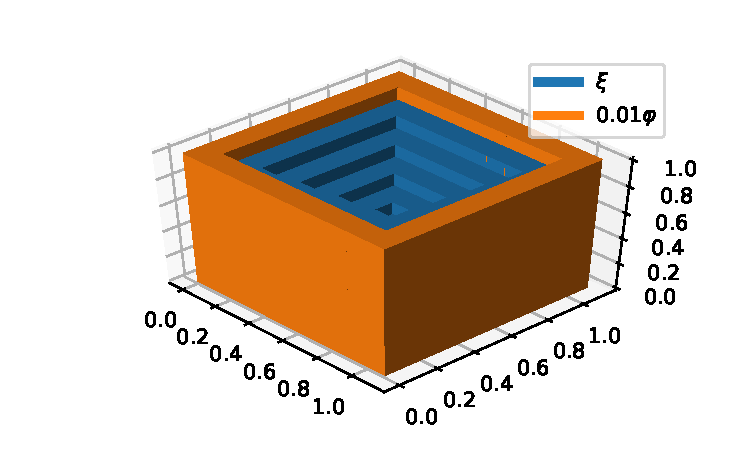
\includegraphics[width=\textwidth]{../img/pdf/collocation_weight.pdf}
	}
	\unterschrift{Weighting factor $\varphi$ and $\xi$ on every collocation point}{}{}
	\label{fig:collocation_weight}
\end{figure}

\begin{table}[h]
	\centering
	\noindent\adjustbox{max width=\linewidth}{
		\begin{tabular}{|c|c|c|}
			
			\hline
			\rowcolor[HTML]{\farbeTabA}
			
			Parameter & JADE & \multilinecell{\cite{chaquet_using_2019}} \\ \hline
			
			$\varphi$ & 100 & 300 \\ \hline
			$\kappa$  & 1   & 3   \\ \hline
			population size & $2 \cdot dim$ & $\frac{3}{2}(4 + \lfloor 3 \cdot ln(dim) \rfloor)$ \\ \hline
			min error & 0   & - \\ \hline
			p & 0.3 & - \\ \hline
			c & 0.5 & - \\ \hline
			replication & 20 & 50 \\ \hline
			\multilinecell{nb \\ nc \\~\\ } & \multilinecell{40 \\ 81 \\ \hline 121 = 11x11}  & \multilinecell{100 equally spaced \\ points over the domain} \\ \hline
			initialisation & $\vec{u_{apx}} \in \mathcal{N}(0,1)$ & \multilinecell{$\omega_i \in \mathcal{U}[-0.01, 0.01]$ \\ $\gamma_i \in \mathcal{U}(0,1]$ \\ $c_{ik} \in \mathcal{U}[2\Omega]$}  \\ \hline
			
		\end{tabular}
	}
	\unterschrift{These predefined parameters are used for the following numerical experiments. }{}{}
	\label{tab:ci_parameter}
\end{table}

\subsection{Hardware Infrastructure}
\label{chap:hardware_setup}
To increase the experimental throughput, two machines are used: a personal computer (machine 1) and a server in the cloud (machine 2). It is important that any time or memory usage comparisons must be performed between experiments on the same machine. In the experiments it is separately denoted which comparisons are allowed. The following table \ref{tab:machines} shows the properties of both machines. It is important to note that these information are only a reference point. This is probably not enough to actually recreate the exact time or memory data presented in this work. Due to the Python incompatibilities, NGSolve can only be installed on machine 1. Thus, any time or memory usage comparisons between the \gls{ci} solver and the \gls{fem} solver must be conducted on machine 1. 
\begin{table}[H]
	\centering
	\noindent\adjustbox{max width=\linewidth}{
		\begin{tabular}{|c|c|c|}
			
			\hline
			\rowcolor[HTML]{\farbeTabA}
			
			Property & Machine 1 & Machine 2 \\ \hline
			
			Operating System & \multilinecell{Windows 10 Home \\ 1909 18363.900} & \multilinecell{CentOS Linux \\ release 7.3.1611} \\ \hline
			Python & \multilinecell{Anaconda version \\ 2019.03} & \multilinecell{Anaconda version \\ 2020.02} \\ \hline
			Processor & \multilinecell{Intel Core i7-4790K \\ CPU @ 4.00GHz} & \multilinecell{Intel Xeon CPU \\ E5-2630 v3 @ 2.40GHz} \\ \hline
			Cores & 4 Cores + 4 logical & 32 Cores \\ \hline
			
		\end{tabular}
	}
	\unterschrift{Comparison of the machines used for the experiments.}{}{}
	\label{tab:machines}
\end{table}
\end{document}